\documentclass{beamer}

% encoding
\usepackage[utf8]{inputenc}
\usepackage[T1]{fontenc}
% language
\usepackage[english]{babel}
% beamer theme
\usetheme{default}
\beamertemplatenavigationsymbolsempty
\hypersetup{pdfpagemode=UseNone} % don't show bookmarks on initial view
% fonts
\usepackage{mathpazo}
\usefonttheme{serif}
% for being able to copy text out of the PDF
\usepackage{cmap}

% math mode formatting etc.
\usepackage{amsmath,amsfonts,amssymb,amsthm,sistyle,xcolor,delim}
\SIstyle{German}
\usepackage{graphicx,tikz,calc,tabularx,hhline}
\usetikzlibrary{backgrounds,calc}

\tikzset{
 >=stealth,
}

% metadata
\title{Training of Hidden Markov models as an instance of the expectation maximization algorithm}
\author{Stefan Majewsky}
\date{22. August 2017}

\begin{document}

\begin{frame}
  \titlepage
\end{frame}

\begin{frame}\frametitle{Gliederung}
 Sprachmodelle
 \begin{itemize}
  \item Bigramm-Modell
  \item Hidden-Markov-Modell
 \end{itemize}
 \pause
 EM-Algorithmen
 \begin{itemize}
  \item Baum-Welch-Algorithmus
  \pause
  \item Inside-Outside-EM-Algorithmus
  \item Instanziierung für Hidden-Markov-Modelle
 \end{itemize}
\end{frame}

\begin{frame}\frametitle{Sprachmodell}
 \begin{itemize}
  \item Ziel: probabilistische Beschreibung einer Sprache
   \[
    \text{Satz } x \mapsto \text{Wahrscheinlichkeit } p(x)
    \vspace{-1em}
   \]
  \pause\item beschrieben durch \emph{Modellparameter} $\omega\in\Omega$
   \[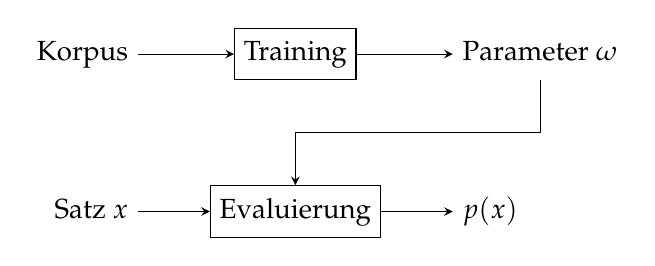
\begin{tikzpicture}[c/.style={rectangle,draw},l/.style={anchor=east},r/.style={anchor=west}]
    \node[l] (corpus)   at (0,+0) { \strut Korpus };
    \node[c] (training) at (2,+0) { \strut Training };
    \node[r] (omega)    at (4,+0) { \strut Parameter $\omega$ };
    \draw[->] (corpus) -- (training);
    \draw[->] (training) -- (omega);
    \node[l] (input)    at (0,-2) { \strut Satz $x$ };
    \node[c] (eval)     at (2,-2) { \strut Evaluierung };
    \node[r] (output)   at (4,-2) { \strut $p(x)$ };
    \draw[->] (input) -- (eval);
    \draw[->] (eval) -- (output);
    \draw[->] (omega.south) |- ($(eval.north)!0.5!(omega.south)$) -| (eval.north);
   \end{tikzpicture}\]
 \end{itemize}
\end{frame}

\begin{frame}\frametitle{Bigramm-Modell}
 \begin{itemize}
  \item Idee: Wahrscheinlichkeit jedes Wortes hängt nur vom vorhergehenden Wort ab
 \end{itemize}
\end{frame}

\end{document}\endinput

Gliederung/Zeitbudget:

- (3 Min) Idee Sprachmodell: P(x), vllt Bigramm-Modell zur Veranschaulichung
- (5 Min) Hidden Markov Model: H = (Q,V,#,t,e) -> P(x)
- (5 Min) Training: Idee Baum-Welch-Algorithmus bzw. EM allgemein -> gute Konvergenz, verallgemeinerbar?
- (10 Min) EM-Algorithmus aus [BSV15]; nur IO-Info, wrsl. eher phänomenologisch (am Beispiel PCFG) als exakt
- (7 Min) Anwendung auf HMM; Bäume aus K bzw. H(x)
